\documentclass[11pt,a4paper]{article}

\usepackage[margin=0.82in]{geometry}
\usepackage[T1]{fontenc}
\usepackage[utf8]{inputenc}
\usepackage{lmodern}
\usepackage{microtype}
\usepackage{graphicx}
\usepackage{booktabs}
\usepackage{array}
\usepackage{longtable}
\usepackage{tabularx}
\usepackage{float}
\usepackage{xcolor}
\usepackage{hyperref}
\usepackage{url}
\usepackage{tikz}
\usetikzlibrary{arrows.meta, positioning, shapes.geometric, fit}

\hypersetup{
  colorlinks=true,
  linkcolor=blue!45!black,
  urlcolor=blue!45!black,
  citecolor=blue!45!black,
  pdftitle={DRISHTI Detailed Project Report},
  pdfauthor={DRISHTI Project}
}

\definecolor{drishtiGreen}{HTML}{19764B}
\definecolor{drishtiRed}{HTML}{B33A3A}
\definecolor{drishtiBlue}{HTML}{2F6FBA}
\definecolor{drishtiGray}{HTML}{555555}
\definecolor{drishtiGold}{HTML}{C77C1A}

\graphicspath{
  {../data/drishti/results/plots/summary/}
  {../data/drishti/results/plots/classified/planet_candidate/}
  {../data/drishti/results/plots/classified/eclipsing_binary/}
  {../data/drishti/results/plots/classified/undetermined/}
}

\newcommand{\code}[1]{\texttt{#1}}
\newcommand{\pct}[1]{#1\%}
\newcommand{\artifact}[1]{\path{#1}}

\title{\textbf{DRISHTI Detailed Project Report}\\
\large Official TESS TCE Recovery, Transit Fitting, Vetting, and Planet-vs-EB Classification}
\author{DRISHTI Project Workspace}
\date{Prepared from current repository artifacts: 19 June 2026}

\begin{document}
\maketitle

\begin{abstract}
DRISHTI (Deep Recognition and Intelligent Screening of Hidden Transit Indicators) is a TESS light-curve recovery and vetting workflow. The work completed so far turns a local set of official TESS Threshold Crossing Events (TCEs) into a reproducible validation pipeline: target selection, light-curve product collection, cleaning, Box Least Squares (BLS) recovery, physical transit fitting, crowded-field and eclipsing-binary vetting, rule-based classification, machine-learning classification, master-catalog generation, and report-grade visualization. The present checkout contains 613 light-curve FITS files, 615 processed candidate-sector rows, a 525-row labeled planet-vs-eclipsing-binary cross-validation set, and a final master catalog with rule and ML classifications. The main scientific result is not a polished planet-discovery claim; it is a defensible validation and triage system. The classifier reaches ROC-AUC 0.94 on the realistic full labeled set, while the default 0.5 threshold gives balanced accuracy 0.80. This means ranking quality is strong, but operating-point selection and additional planet labels remain the key next steps.
\end{abstract}

\tableofcontents
\listoffigures
\listoftables
\newpage

\section{Executive Summary}

The project has progressed from a raw TESS-data workspace into an end-to-end DRISHTI validation pipeline. The active question is:

\begin{quote}
Can the pipeline recover known official TESS TCE signals, measure them, and decide whether each signal is planet-like, eclipsing-binary-like, blended, or too uncertain to classify?
\end{quote}

\noindent The answer so far is: yes, the pipeline works as a validation and triage system. It is not yet a finished blind planet-discovery engine. That distinction matters. The workflow now produces machine-readable evidence tables, interpretable classifications, trained ML probabilities, diagnostic plots, and summary figures.

\begin{table}[H]
\centering
\caption{Current project state at a glance.}
\begin{tabular}{@{}lr@{}}
\toprule
Quantity & Current value \\
\midrule
LC FITS files stored under \artifact{data/drishti/downloads/lc/} & 613 \\
Starter validation target-sector rows & 111 \\
Labeled training target-sector rows & 504 \\
Total processed candidate-sector rows in master catalog & 615 \\
Unique TIC IDs in master catalog & 516 \\
Full labeled ML cross-validation rows & 525 \\
Planets in full ML CV set & 66 \\
Eclipsing binaries in full ML CV set & 459 \\
ML ROC-AUC on full labeled set & 0.94 \\
ML balanced accuracy at threshold 0.5 & 0.80 \\
\bottomrule
\end{tabular}
\end{table}

The most important lesson is that the earlier balanced labeled set was optimistic. When the EB sample was expanded to a more realistic prevalence, planet precision and recall fell, but ROC-AUC stayed high. The system still ranks candidates well; the default decision threshold is simply not the best scientific operating point for rare planets.

\section{Repository and Artifact Layout}

The active generated-data root is \artifact{data/drishti/}. Older results under \artifact{outputs/} are legacy or model-only artifacts, except for the trained model at \artifact{outputs/models/planet_eb_rf.joblib}.

\begin{figure}[H]
\centering
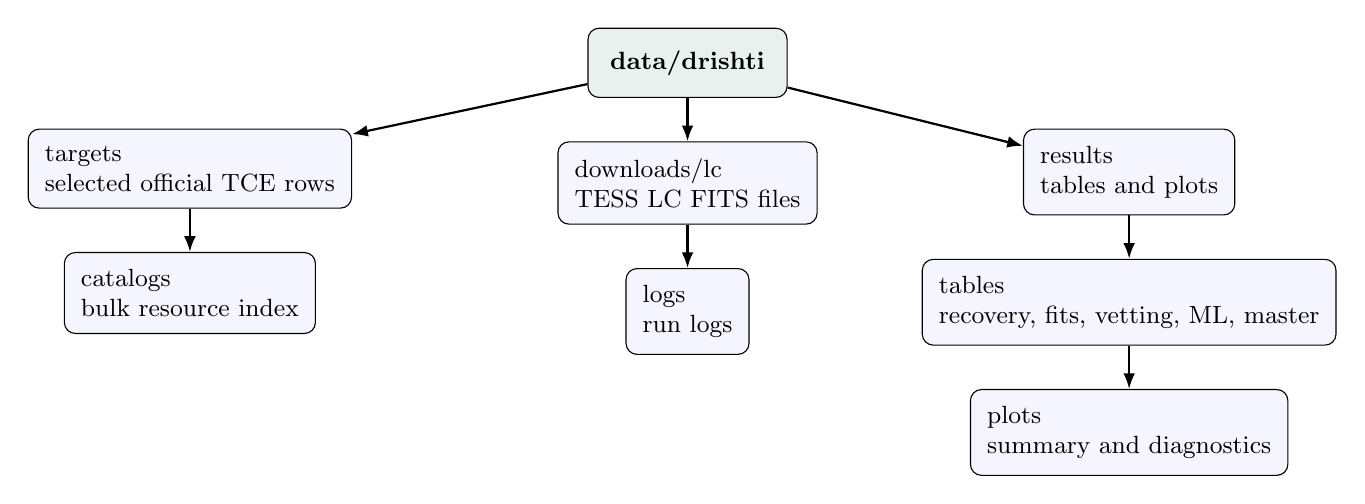
\begin{tikzpicture}[
  node distance=0.55cm,
  box/.style={draw, rounded corners, align=left, fill=blue!4, inner sep=6pt, font=\small},
  root/.style={draw, rounded corners, align=center, fill=drishtiGreen!10, inner sep=8pt, font=\small\bfseries},
  arr/.style={-{Latex[length=2mm]}, thick}
]
\node[root] (root) {data/drishti};
\node[box, below left=of root, xshift=-2.6cm] (targets) {targets\\selected official TCE rows};
\node[box, below=of root] (downloads) {downloads/lc\\TESS LC FITS files};
\node[box, below right=of root, xshift=2.6cm] (results) {results\\tables and plots};
\node[box, below=of targets] (catalogs) {catalogs\\bulk resource index};
\node[box, below=of downloads] (logs) {logs\\run logs};
\node[box, below=of results] (tables) {tables\\recovery, fits, vetting, ML, master};
\node[box, below=of tables] (plots) {plots\\summary and diagnostics};
\draw[arr] (root) -- (targets);
\draw[arr] (root) -- (downloads);
\draw[arr] (root) -- (results);
\draw[arr] (targets) -- (catalogs);
\draw[arr] (downloads) -- (logs);
\draw[arr] (results) -- (tables);
\draw[arr] (tables) -- (plots);
\end{tikzpicture}
\caption{Canonical DRISHTI storage layout used by the current pipeline.}
\end{figure}

\begin{table}[H]
\centering
\caption{Main result files and what they contain.}
\begin{tabularx}{\textwidth}{@{}lX@{}}
\toprule
Artifact & Purpose \\
\midrule
\artifact{data/drishti/results/tables/master_candidates.csv} & Final joined catalog with recovery class, fitted parameters, noise context, rule class, confidence, label, and ML planet probability. \\
\artifact{data/drishti/results/tables/tce_recovery_results_111.csv} & Starter official-TCE recovery benchmark. \\
\artifact{data/drishti/results/tables/tce_recovery_results_labeled.csv} & Recovery results for the labeled training expansion. \\
\artifact{data/drishti/results/tables/transit_fits_111.csv} & Transit-fit parameters and uncertainties for the starter set. \\
\artifact{data/drishti/results/tables/transit_fits_labeled.csv} & Transit-fit parameters and uncertainties for the labeled expansion. \\
\artifact{data/drishti/results/tables/vetting_features_labeled.csv} & Centroid, crowding, odd-even, secondary, shape, and duration vetting features for labeled targets. \\
\artifact{data/drishti/results/tables/ml_classification_cv_full.csv} & Cross-validated ML predictions for the 525-row full labeled set. \\
\artifact{data/drishti/results/plots/summary/} & Report-level figures: recovery, depth accuracy, ROC, confusion, reliability, feature importances. \\
\artifact{data/drishti/results/plots/classified/} & Per-candidate diagnostic plots grouped by predicted rule class. \\
\bottomrule
\end{tabularx}
\end{table}

\section{End-to-End Workflow}

The implemented DRISHTI workflow is shown in Figure~\ref{fig:workflow}. The important design choice is that the project validates against known official TCEs before claiming blind discovery performance.

\begin{figure}[H]
\centering
\begin{tikzpicture}[
  node distance=0.55cm,
  step/.style={draw, rounded corners, align=center, fill=gray!5, minimum width=3.7cm, minimum height=0.85cm, font=\small},
  evidence/.style={draw, rounded corners, align=center, fill=drishtiGreen!8, minimum width=3.7cm, minimum height=0.85cm, font=\small},
  output/.style={draw, rounded corners, align=center, fill=drishtiBlue!8, minimum width=3.7cm, minimum height=0.85cm, font=\small},
  arr/.style={-{Latex[length=2mm]}, thick}
]
\node[step] (targets) {Official TCE target lists};
\node[step, below=of targets] (download) {LC FITS download/load};
\node[step, below=of download] (clean) {Clean and flatten light curve};
\node[step, below=of clean] (bls) {BLS transit search};
\node[evidence, below=of bls] (recover) {Compare to official period, epoch, duration, SNR};
\node[evidence, below left=of recover, xshift=-2.3cm] (fit) {Trapezoid transit fit\\depth, duration, uncertainty};
\node[evidence, below right=of recover, xshift=2.3cm] (vet) {Vetting evidence\\centroid, EB tests, shape};
\node[output, below=of recover, yshift=-2.5cm] (classify) {Rule + ML classification};
\node[output, below=of classify] (catalog) {Master catalog and plots};
\draw[arr] (targets) -- (download);
\draw[arr] (download) -- (clean);
\draw[arr] (clean) -- (bls);
\draw[arr] (bls) -- (recover);
\draw[arr] (recover) -- (fit);
\draw[arr] (recover) -- (vet);
\draw[arr] (fit) -- (classify);
\draw[arr] (vet) -- (classify);
\draw[arr] (classify) -- (catalog);
\end{tikzpicture}
\caption{Implemented DRISHTI workflow from official TCE rows to final candidate products.}
\label{fig:workflow}
\end{figure}

\subsection{Target Selection}

Target lists are built from local official TCE reference tables under \artifact{data/Ref/}. The selected target schema preserves scientific provenance:

\begin{itemize}
  \item \code{tic_id} and \code{sector}
  \item \code{official_period}
  \item \code{official_epoch}
  \item \code{official_duration_hours}
  \item \code{official_depth}
  \item \code{official_snr}
  \item \code{official_num_transits}
  \item \code{official_full_convergence}
  \item \code{source_tce_file}
\end{itemize}

\begin{table}[H]
\centering
\caption{Current target-list sizes.}
\begin{tabular}{@{}lr@{}}
\toprule
Target list & Rows \\
\midrule
\artifact{tce_starter_validation_targets.csv} & 111 \\
\artifact{tce_positive_targets.csv} & 1538 \\
\artifact{labeled_training_targets.csv} & 504 \\
\artifact{labeled_highvalue_targets.csv} & 101 \\
\artifact{tce_recovery_batch_50.csv} & 50 \\
\artifact{tce_recovery_batch_111.csv} & 111 \\
\bottomrule
\end{tabular}
\end{table}

\subsection{Light-Curve Products}

The current checkout contains 613 TESS light-curve FITS files under \artifact{data/drishti/downloads/lc/}. The result tables cover 615 candidate-sector rows: 111 starter rows and 504 labeled-training rows. The two-row difference is accounted for in the labeled run as missing LC FITS products.

\begin{table}[H]
\centering
\caption{Processing coverage from current artifacts.}
\begin{tabular}{@{}lrr@{}}
\toprule
Stage & Rows & Notes \\
\midrule
LC FITS files on disk & 613 & Stored under \artifact{downloads/lc/}. \\
Starter recovery rows & 111 & All have transit fits. \\
Labeled recovery rows & 504 & 502 fit OK, 2 missing LC FITS. \\
Master-catalog rows & 615 & 111 starter + 504 labeled rows. \\
Unique TIC IDs in master catalog & 516 & Multiple sector rows exist for some TICs. \\
\bottomrule
\end{tabular}
\end{table}

\section{Detection and Recovery}

\subsection{BLS Recovery Logic}

For each target-sector row, DRISHTI loads the LC FITS product, cleans and flattens the light curve, runs BLS, and compares the strongest recovered signal with the official TCE. The recovery classification uses:

\begin{itemize}
  \item period error against official TCE period,
  \item harmonic checks for half-period and double-period aliases,
  \item phase or epoch alignment against official epoch,
  \item duration ratio against official duration,
  \item BLS SNR threshold.
\end{itemize}

This produces more information than a single pass/fail flag. For example, \code{period_recovered_bad_duration} indicates a period match with suspicious duration, and \code{period_recovered_epoch_mismatch} indicates a period match with poor phase agreement.

\subsection{Starter Validation Results}

\begin{table}[H]
\centering
\caption{Starter 111-row official-TCE recovery benchmark.}
\begin{tabular}{@{}lrr@{}}
\toprule
Recovery class & Count & Fraction of 111 \\
\midrule
\code{direct_recovered} & 76 & \pct{68.5} \\
\code{alias_recovered} & 4 & \pct{3.6} \\
\code{period_recovered_bad_duration} & 5 & \pct{4.5} \\
\code{period_recovered_epoch_mismatch} & 4 & \pct{3.6} \\
\code{not_recovered} & 22 & \pct{19.8} \\
\midrule
Direct or alias recovered & 80 & \pct{72.1} \\
Period recovered or vetting-worthy & 89 & \pct{80.2} \\
\bottomrule
\end{tabular}
\end{table}

\begin{figure}[H]
\centering
\includegraphics[width=0.92\textwidth]{recovery_classes.png}
\caption{Recovery-class distribution across the combined 615-row processed evidence set.}
\label{fig:recovery-classes}
\end{figure}

\subsection{Labeled Expansion Recovery Results}

The labeled expansion was used to create a much stronger planet-vs-EB classifier. It is more diverse and more EB-heavy than the starter validation set.

\begin{table}[H]
\centering
\caption{Recovery classes for the 504-row labeled-training expansion.}
\begin{tabular}{@{}lr@{}}
\toprule
Recovery class & Count \\
\midrule
\code{direct_recovered} & 182 \\
\code{alias_recovered} & 125 \\
\code{period_recovered_epoch_mismatch} & 28 \\
\code{period_recovered_bad_duration} & 15 \\
\code{period_recovered_needs_vetting} & 8 \\
\code{not_recovered} & 144 \\
\code{download_failed} & 2 \\
\midrule
Direct or alias recovered & 307 \\
Period recovered or vetting-worthy & 358 \\
\bottomrule
\end{tabular}
\end{table}

\section{Transit Fitting and Parameter Accuracy}

DRISHTI fits a symmetric trapezoid transit model to the phase-folded light curve. The fit reports period, epoch, depth, duration, ingress fraction, uncertainties, reduced chi-square, and BIC. A key improvement was the switch to a transit-masked second detrending pass for fitting. Without that step, the flattening window could absorb part of the transit depth.

\begin{table}[H]
\centering
\caption{Transit-fit status and median parameter ratios.}
\begin{tabular}{@{}lrrr@{}}
\toprule
Table & Fit OK & Median depth ratio & Median duration ratio \\
\midrule
\artifact{transit_fits_111.csv} & 111 / 111 & 0.924 & 0.962 \\
\artifact{transit_fits_labeled.csv} & 502 / 504 & 0.920 & 0.982 \\
\bottomrule
\end{tabular}
\end{table}

\begin{figure}[H]
\centering
\includegraphics[width=0.76\textwidth]{depth_accuracy.png}
\caption{Fitted transit depth versus official TCE depth. The median fitted-to-official depth ratio is approximately 0.92.}
\label{fig:depth}
\end{figure}

\begin{table}[H]
\centering
\caption{Starter-set parameter accuracy by recovery class.}
\begin{tabular}{@{}lrrr@{}}
\toprule
Recovery class & $n$ & Median depth ratio & Median duration ratio \\
\midrule
\code{direct_recovered} & 76 & 0.935 & 0.972 \\
\code{alias_recovered} & 4 & 1.214 & 2.551 \\
\code{period_recovered_bad_duration} & 5 & 0.857 & 4.777 \\
\code{period_recovered_epoch_mismatch} & 4 & 0.414 & 1.056 \\
\code{not_recovered} & 22 & 0.574 & 0.804 \\
\bottomrule
\end{tabular}
\end{table}

The direct-recovered class is the cleanest measurement regime. Alias and partial-recovery classes degrade in physically interpretable ways, which confirms that the recovery taxonomy is meaningful rather than cosmetic.

\section{Vetting Evidence}

The vetting layer is designed to answer the question: even if a transit-like dip exists, does it look like a planet, an eclipsing binary, a blend, or an uncertain event?

\subsection{Vetting Features}

The current evidence vector includes:

\begin{itemize}
  \item \code{CROWDSAP} and \code{FLFRCSAP} aperture contamination context,
  \item in-transit versus out-of-transit centroid shift,
  \item odd-even transit-depth consistency,
  \item secondary-eclipse SNR and secondary-to-primary ratio,
  \item local V-shape versus U-shape metric,
  \item duration sanity ratio,
  \item aggregate \code{blend_flag} and \code{eb_flag}.
\end{itemize}

\begin{table}[H]
\centering
\caption{Blend and EB vetting summaries.}
\begin{tabular}{@{}llr@{}}
\toprule
Set & Flag & Count \\
\midrule
Starter 111 & \code{on_target} & 109 \\
Starter 111 & \code{crowded_on_target} & 2 \\
Starter 111 & \code{eb_suspect} & 36 \\
Starter 111 & \code{v_shaped_watch} & 42 \\
Starter 111 & \code{ok} & 33 \\
\midrule
Labeled 504 & \code{on_target} & 464 \\
Labeled 504 & \code{crowded_on_target} & 13 \\
Labeled 504 & \code{unknown blend} & 27 \\
Labeled 504 & \code{eb_suspect} & 172 \\
Labeled 504 & \code{v_shaped_watch} & 135 \\
Labeled 504 & \code{ok} & 195 \\
\bottomrule
\end{tabular}
\end{table}

The vetting layer is important because it gives physically explainable reasons for classification. A model probability alone is not enough for scientific review; DRISHTI preserves the underlying evidence.

\section{Classification}

\subsection{Rule-Based Classification}

The transparent rule-based classifier assigns:

\begin{itemize}
  \item \code{planet_candidate},
  \item \code{eclipsing_binary},
  \item \code{blend},
  \item \code{undetermined}.
\end{itemize}

Each row carries \code{rule_class}, \code{rule_confidence}, and \code{rule_reason}. The rule layer is not meant to be perfect; it is meant to be inspectable and scientifically traceable.

\begin{table}[H]
\centering
\caption{Rule-based classes in the 615-row master catalog.}
\begin{tabular}{@{}lr@{}}
\toprule
Rule class & Count \\
\midrule
\code{planet_candidate} & 279 \\
\code{eclipsing_binary} & 160 \\
\code{undetermined} & 176 \\
\bottomrule
\end{tabular}
\end{table}

\subsection{Label Assembly and ML Training Set}

The ML classifier is trained and validated on rows with bootstrapped labels from TOI/ExoFOP-style planet labels and TESS EB labels. The final cross-validation set contains 525 trainable rows.

\begin{table}[H]
\centering
\caption{Class labels in the master catalog and final trainable ML subset.}
\begin{tabular}{@{}lrr@{}}
\toprule
Label & Master catalog count & Used in final planet-vs-EB CV \\
\midrule
\code{eclipsing_binary} & 459 & 459 \\
\code{planet} & 66 & 66 \\
\code{planet_candidate} & 38 & 0 \\
\code{false_positive} & 15 & 0 \\
Unlabeled & 37 & 0 \\
\bottomrule
\end{tabular}
\end{table}

\subsection{Full 525-Row Classifier Result}

The full ML result is the honest operating picture. The classifier is a class-weight-balanced RandomForest evaluated using stratified cross-validation. At the default threshold of 0.5:

\begin{table}[H]
\centering
\caption{Full 525-row ML classifier metrics.}
\begin{tabular}{@{}lr@{}}
\toprule
Metric & Value \\
\midrule
ROC-AUC & 0.944 \\
Balanced accuracy & 0.795 \\
EB precision & 0.949 \\
EB recall & 0.939 \\
EB F1 & 0.944 \\
Planet precision & 0.606 \\
Planet recall & 0.652 \\
Planet F1 & 0.628 \\
\bottomrule
\end{tabular}
\end{table}

\begin{table}[H]
\centering
\caption{Confusion matrix at ML threshold 0.5. Rows are true class and columns are predicted class.}
\begin{tabular}{@{}lrr@{}}
\toprule
True class & Predicted EB & Predicted planet \\
\midrule
Eclipsing binary & 431 & 28 \\
Planet & 23 & 43 \\
\bottomrule
\end{tabular}
\end{table}

\begin{figure}[H]
\centering
\includegraphics[width=0.72\textwidth]{ml_roc.png}
\caption{Cross-validated ROC curve for the full 525-row planet-vs-EB classifier.}
\label{fig:roc}
\end{figure}

\begin{figure}[H]
\centering
\includegraphics[width=0.66\textwidth]{ml_confusion.png}
\caption{Cross-validated confusion matrix at the default threshold of 0.5.}
\label{fig:confusion}
\end{figure}

\subsection{Probability Calibration and Operating Point}

The main nuance is threshold selection. The earlier balanced 122-row set made the classifier look cleaner than it is under realistic prevalence. The full 525-row set has many more EBs, and many EBs resemble planets. That is why planet precision and recall fall at the default threshold.

\begin{table}[H]
\centering
\caption{Cross-validated probability bins on the full labeled set.}
\begin{tabular}{@{}lrr@{}}
\toprule
ML planet probability bin & Rows & Actual planet fraction \\
\midrule
$[0.00, 0.25)$ & 367 & 0.014 \\
$[0.25, 0.50)$ & 87 & 0.207 \\
$[0.50, 0.75)$ & 41 & 0.415 \\
$[0.75, 1.00]$ & 30 & 0.867 \\
\bottomrule
\end{tabular}
\end{table}

\begin{figure}[H]
\centering
\includegraphics[width=0.96\textwidth]{ml_reliability.png}
\caption{Reliability curve and score distribution. The useful scientific action is to choose an operating threshold rather than treating 0.5 as sacred.}
\label{fig:reliability}
\end{figure}

The interpretation is positive but cautious. ROC-AUC 0.94 means the model ranks planets above EBs well. However, a default 0.5 cutoff is not necessarily the right threshold when planets are scarce. A high-purity planet shortlist should use a higher probability threshold and then inspect the classified plots.

\begin{figure}[H]
\centering
\includegraphics[width=0.86\textwidth]{feature_importances.png}
\caption{RandomForest feature importances. Top features are physically meaningful: fitted depth, centroid shift, secondary-eclipse SNR, ingress fraction, duration sanity, shape, BLS period, and BLS SNR.}
\label{fig:features}
\end{figure}

\section{Diagnostic Visualizations}

Per-candidate plots are generated under \artifact{data/drishti/results/plots/classified/}. They combine the cleaned time-domain light curve, shaded transit windows, phase-folded signal, fitted trapezoid model, rule class, rule confidence, ML planet probability, and known label when available.

\begin{figure}[H]
\centering
\includegraphics[width=\textwidth]{TIC_25155310_S0001_classified.png}
\caption{Example candidate classified as planet-like.}
\end{figure}

\begin{figure}[H]
\centering
\includegraphics[width=\textwidth]{TIC_38937499_S0002_classified.png}
\caption{Example candidate classified as eclipsing-binary-like.}
\end{figure}

\begin{figure}[H]
\centering
\includegraphics[width=\textwidth]{TIC_150187916_S0002_classified.png}
\caption{Example candidate classified as undetermined. These plots are essential for reviewing borderline cases.}
\end{figure}

\section{What Has Been Built}

\begin{longtable}{@{}p{0.28\textwidth}p{0.66\textwidth}@{}}
\caption{Implemented project components.}\\
\toprule
Component & Status and role \\
\midrule
\endfirsthead
\toprule
Component & Status and role \\
\midrule
\endhead
Centralized DRISHTI store & Implemented via \artifact{src/drishti_store.py}. Active artifact root is \artifact{data/drishti/}. \\
Official TCE target selection & Implemented in \artifact{scripts/select_tce_targets.py}; preserves official period, epoch, duration, depth, SNR, convergence, transit count, and source file. \\
Download and manifest workflow & Implemented in \artifact{scripts/drishti.py} and \artifact{scripts/05_download_tce_products.py}; current LC FITS store contains 613 files. \\
BLS recovery benchmark & Implemented in \artifact{scripts/06_run_tce_recovery.py} and integrated into the CLI; starter 111 benchmark is complete. \\
Transit fitting & Implemented in \artifact{src/fitting/transit_fit.py} and \artifact{scripts/08_fit_transits.py}; includes depth and duration uncertainties. \\
Vetting evidence & Implemented under \artifact{src/vetting/} and \artifact{scripts/09_run_vetting.py}; includes centroid, crowding, odd-even, secondary, shape, and duration checks. \\
Rule-based classifier & Implemented in \artifact{src/models/classifier.py} and \artifact{scripts/10_classify_candidates.py}; produces transparent class reasons. \\
Label assembly & Implemented in \artifact{scripts/get_labels.py}; creates bootstrapped labels for ML training and validation. \\
ML classifier & Implemented in \artifact{scripts/11_train_classifier.py}; final full CV table has 525 rows and ROC-AUC 0.94. \\
Master catalog & Implemented in \artifact{scripts/12_finalize_candidates.py}; final catalog has 615 rows. \\
Candidate plots & Implemented in \artifact{scripts/13_plot_classified.py}; plots grouped by predicted class. \\
Summary plots & Implemented in \artifact{scripts/14_plot_summary.py}; six report-level plots are present. \\
Workflow guide & Implemented in \artifact{docs/DRISHTI_WORKFLOW_GUIDE.md}. \\
\bottomrule
\end{longtable}

\section{How To Reproduce the Main Outputs}

\subsection{Environment}

\begin{verbatim}
.\.venv\Scripts\Activate.ps1
\end{verbatim}

\subsection{Run the Full Labeled Evidence Processor}

\begin{verbatim}
python .\scripts\process_targets_parallel.py `
  --targets .\data\drishti\targets\labeled_training_targets.csv `
  --suffix labeled `
  --workers 14
\end{verbatim}

\subsection{Train the Full Classifier}

\begin{verbatim}
python .\scripts\11_train_classifier.py `
  --recovery .\data\drishti\results\tables\tce_recovery_results_111.csv `
             .\data\drishti\results\tables\tce_recovery_results_labeled.csv `
  --fits .\data\drishti\results\tables\transit_fits_111.csv `
         .\data\drishti\results\tables\transit_fits_labeled.csv `
  --vetting .\data\drishti\results\tables\vetting_features_111.csv `
            .\data\drishti\results\tables\vetting_features_labeled.csv `
  --pred-out .\data\drishti\results\tables\ml_classification_cv_full.csv
\end{verbatim}

\subsection{Build Final Catalog and Plots}

\begin{verbatim}
python .\scripts\12_finalize_candidates.py
python .\scripts\13_plot_classified.py --per-class 5
python .\scripts\14_plot_summary.py
\end{verbatim}

\section{Interpretation}

The work was not a waste. It changed the project from an idea into a measurable pipeline. The full result is scientifically more useful than an inflated number because it exposes the real operating difficulty:

\begin{itemize}
  \item Official-TCE recovery works and is quantified.
  \item Transit fitting is physically reasonable after correcting depth suppression.
  \item Vetting features carry meaningful astrophysical information.
  \item EB-heavy realistic validation lowers planet precision and recall at threshold 0.5.
  \item ROC-AUC remains high, so candidate ranking is strong.
  \item The next decision is the operating point: high-purity shortlist versus higher planet recall.
\end{itemize}

In practical terms, DRISHTI is currently best described as a validation and triage engine. It can produce ranked candidate shortlists and explain why a candidate looks planet-like or EB-like. It is not yet a final blind discovery system.

\section{Limitations}

\begin{itemize}
  \item Planet labels are still scarce: only 66 confirmed planet rows are in the full ML CV set.
  \item Labels are bootstrapped from available catalogs, not a manually curated gold-standard training set.
  \item The ML classifier is binary planet-vs-EB; blends remain handled by rule and centroid evidence rather than a trained blend class.
  \item Performance on a blind science sector has not yet been validated.
  \item Target-pixel-level difference imaging is not yet integrated into the main report result.
  \item Threshold 0.5 is a default, not a scientifically optimized decision boundary.
\end{itemize}

\section{Recommended Next Steps}

\begin{enumerate}
  \item Choose an operating threshold for \code{ml_planet_proba}. For example, tune for a high-purity shortlist first.
  \item Inspect all high-probability planet candidates using the classified plots.
  \item Expand confirmed planet labels beyond 66 rows.
  \item Run a blind-sector test and compare the resulting shortlist against known TOIs and EBs.
  \item Add target-pixel or DV-product evidence for stronger blend rejection.
  \item Convert this LaTeX report into the formal final report style after the blind-sector result is added.
\end{enumerate}

\appendix
\section{Numerical Inventory}

\begin{table}[H]
\centering
\caption{CSV row-count inventory from the current result table directory.}
\begin{tabular}{@{}lr@{}}
\toprule
CSV file & Rows \\
\midrule
\artifact{candidate_classifications_111.csv} & 111 \\
\artifact{labeled_download_status.csv} & 504 \\
\artifact{master_candidates.csv} & 615 \\
\artifact{ml_classification_cv.csv} & 67 \\
\artifact{ml_classification_cv_expanded.csv} & 122 \\
\artifact{ml_classification_cv_full.csv} & 525 \\
\artifact{tce_download_status_111.csv} & 111 \\
\artifact{tce_recovery_results_111.csv} & 111 \\
\artifact{tce_recovery_results_labeled.csv} & 504 \\
\artifact{transit_fits_111.csv} & 111 \\
\artifact{transit_fits_labeled.csv} & 504 \\
\artifact{vetting_features_111.csv} & 111 \\
\artifact{vetting_features_labeled.csv} & 504 \\
\bottomrule
\end{tabular}
\end{table}

\section{Key Paths}

\begin{itemize}
  \item Report source: \artifact{report/drishti_detailed_report.tex}
  \item Existing Markdown report: \artifact{report/REPORT.md}
  \item Workflow guide: \artifact{docs/DRISHTI_WORKFLOW_GUIDE.md}
  \item Master catalog: \artifact{data/drishti/results/tables/master_candidates.csv}
  \item Summary plots: \artifact{data/drishti/results/plots/summary/}
  \item Classified plots: \artifact{data/drishti/results/plots/classified/}
\end{itemize}

\end{document}
